\chapter{Literature Review}

\section{Bond Theory and the Bond Model}

\subsection{Background on Bond}
The structural performance of reinforced concrete fundamentally depends on the ability of embedded steel reinforcing bars to transfer forces to and from the surrounding concrete matrix. This force transfer mechanism, broadly referred to as 'bond', governs how tensile and compressive stresses develop along a bar's length, dictates anchorage and development length requirements, and influences crack spacing, crack width, and deformation behaviour at the member level. A thorough understanding of bond theory is therefore a prerequisite for the development of any bond model or analytically derived development length equation. This chapter reviews the fundamental definition and theoretical background of bond, the mechanisms of bond resistance, the modes of bond failure, and the principal predictive models that have been proposed in the literature.

Bond in reinforced concrete is defined as the interfacial interaction between the surface of an embedded reinforcing bar and the surrounding concrete that enables the transfer of longitudinal forces between the two materials. It is quantified as the bond stress ($\tau$), defined as the shear stress per unit of nominal bar surface area acting parallel to the bar axis at the steel-concrete interface. For a bar of diameter $d_b$ embedded over a length $L$ and subject to a tensile force $P$, the average bond stress is given by:

\begin{equation}
\tau = \frac{P}{\pi d_b L}
\end{equation}

In reality, bond stress is non-uniformly distributed along the anchorage length. It peaks near the loaded end of the bar and diminishes toward the free end, with the exact distribution depending on the local bond-slip constitutive relationship, the strain distribution in the bar, and the degree of confinement provided by the concrete cover and transverse reinforcement (Tepfers, 1973; fib Model Code 2010, 2013). This non-uniformity has important implications for the definition of development length rather than being a simple product of average bond stress and perimeter, development length must be derived from integration of the local bond-slip law along the bar, a process that underpins the analytical development length approach pursued in the present thesis.

For deformed reinforcing bars, the total bond resistance between bar and concrete arises from three distinct physical mechanisms, each active at different stages of loading and slip \parencite{408R03BondDevelopment} (ACI 408R-03, 2003; Tepfers, 1973):
\begin{itemize}
  \item \textbf{Chemical adhesion} – molecular attraction between the concrete and the steel surface; significant only at the very first stage of loading when slip is negligible.
  \item \textbf{Mechanical interlock} – bearing of the ribs (or deformations) on the concrete “keys” that form between adjacent ribs. For deformed bars, mechanical interlock dominates the bond capacity, providing far higher resistance than adhesion or friction alone.
  \item \textbf{Friction} – resistance generated by the normal pressure acting on the bar surface and by the roughness of the concrete.
\end{itemize}

\begin{figure}[H]
    \centering
    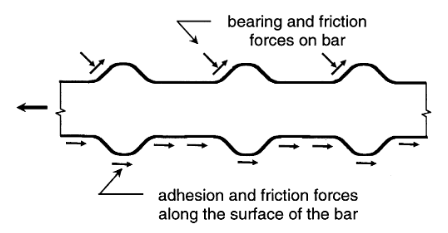
\includegraphics[width=0.7\textwidth]{bond_transfer_mech.png}
    \caption{Schematic of bond transfer mechanisms in reinforced concrete (ACI 408R-03, 2003).}
    \label{fig:bond_transfer_mech}
\end{figure}

The relative magnitudes of these three components, and the slip levels at which they are mobilised, vary with bar surface geometry, concrete strength, cover, and confinement. For practical reinforced concrete design with deformed bars, mechanical interlock accounts for the large majority of total bond resistance and is the mechanism captured by the constitutive parameters in bond-slip models such as the fib Model Code 2010. 

\newpage
\subsection{Failure Modes}
\subsubsection{Pull-Out Failure}
Pull-out failure occurs when the concrete keys between ribs are sheared off, allowing the bar to slide axially without splitting the cover. It governs under well-confined conditions, large cover ($c/d_{b}$ $\gtrsim$ 2.5-3.0) or dense transverse reinforcement, where hoop stresses are suppressed below the splitting threshold. The response is ductile: bond stress peaks at a slip of approximately 1–3 mm then declines gradually to a friction residual. The fib MC 2010 expresses peak bond stress as ${\tau }_{max}\ =\ 2.5\sqrt{f_{c}}$ (MPa) for well-confined bars. Foster et al. (2024) observed pull-out as the governing mode in all 54 SENSE600 Stage II specimens at $20d_b$ with helical confinement.

\subsubsection{Splitting Failure}
Splitting failure occurs when radial rib bearing forces generate hoop tensile stresses that exceed the concrete tensile capacity, driving longitudinal cracks through the cover. Once the crack reaches the external surface, bond resistance drops suddenly and the failure is brittle. This mode dominates in practice where cover is limited and transverse reinforcement is sparse, the typical situation in slabs and footings. Two geometries are recognised depending on bar arrangement: face-and-side splitting, governed by the minimum of side cover and half the clear bar spacing; and bottom splitting, governed by bottom cover. AS3600 and Eurocode 2 select the governing dimension accordingly. The transition between modes is gradual: increasing cover or reducing bar diameter favours pull-out, while very high-strength concrete can promote splitting at lower cover ratios due to the brittle fracture of the matrix (Harajli, 2004).

\begin{figure}[H]
    \centering
    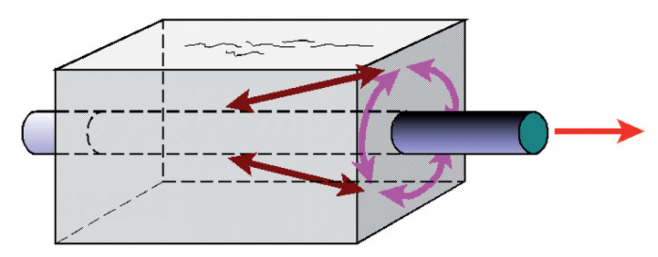
\includegraphics[width=0.7\textwidth]{splitting cairns.png}
    \caption{Schematic of splitting failure in reinforced concrete (Cairns, 2013).}
    \label{fig:splitting_failure}
\end{figure}

\subsection{Factors Influencing Bond Strength}
Bond strength is governed by the interaction of several material and geometric factors. This section summarises the key factors identified consistently across the experimental literature, with reference to \textcite{liTensileBondAnchorage2012}, whose systematic program on Australian 500N bars provides the most comprehensive single-source dataset for the Australian context and the direct experimental baseline for SENSE600 comparison.

\subsubsection{Concrete Compressive Strength}

Bond strength increases with concrete compressive strength, as higher-strength concrete provides greater resistance to both rib bearing (pull-out capacity) and hoop tension (splitting resistance). However, this relationship is non-linear: as concrete grade increases beyond approximately 40 MPa, the incremental benefit on bond diminishes because the fracture mode transitions from aggregate debonding toward aggregate splitting, where the matrix toughness grows more slowly than compressive strength. Darwin (2005) and ACI 408R-03 (2003) demonstrated that ${{f^{\prime }}_{c}}^{0.25}$ better represents the concrete contribution to bond than the traditionally used ${{f^{\prime }}_{c}}^{0.5}$ for unconfined bars across the full practical range of concrete strengths. \textcite{liTensileBondAnchorage2012} confirmed this in their regression for Australian 500N bars:

\begin{equation}
\tau_u = 23.315{{f^{\prime }}_{c}}^{0.25} -37.579
\end{equation}
using the fourth-root term throughout their analysis of all five influencing factors.

\begin{figure}[H]
    \centering
    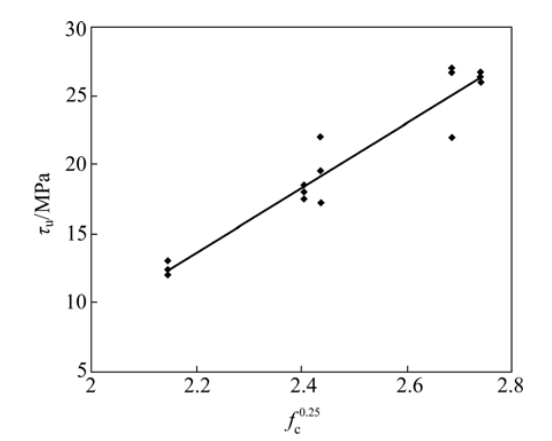
\includegraphics[width=0.6\textwidth]{tensile vs bond strength .png}
    \caption{Relationship between concrete tensile strength and bond strength \parencite{liTensileBondAnchorage2012}.}
    \label{fig:tensile_bond_strength}
\end{figure}

\subsubsection{Bar Diameter}
Bond strength per unit area decreases with increasing bar diameter. Larger bars carry proportionally greater tensile forces relative to their bonded surface area, generate more non-uniform bond stress distributions over longer required embedment lengths, and produce greater radial bearing forces that increase the risk of splitting. \textcite{liTensileBondAnchorage2012} quantified this for Australian 500N bars through their Group BL tests across diameters from 8 to 36 mm, expressing the normalised bond strength as: 

\begin{equation}
\frac{\tau_u}{{f^{\prime}_{c}}^{0.25}} = \frac{83.043}{d^{0.5592}}
\end{equation}

This size effect is codified through the $k_{2}$ factor in AS3600 and the ${\eta }_{3}$ factor in fib MC2010.

\begin{figure}[H]
    \centering
    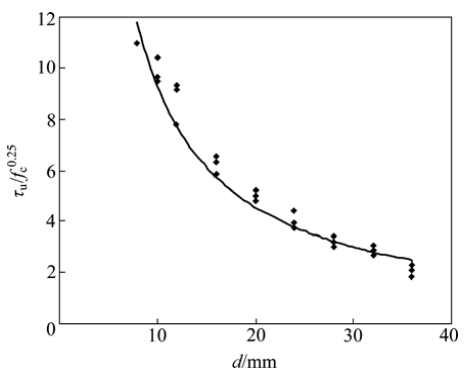
\includegraphics[width=0.6\textwidth]{tensile vs db.png}
    \caption{Relationship between concrete tensile strength and bar diameter \parencite{liTensileBondAnchorage2012}.}
    \label{fig:tensile_db}
\end{figure}

\subsubsection{Concrete Cover}
Increasing concrete cover raises bond strength by providing greater confinement against the radial bearing forces of the ribs, delaying the initiation and propagation of splitting cracks and allowing more of the concrete's tensile capacity to be mobilised before failure. \textcite{liTensileBondAnchorage2012} demonstrated a clear and consistent increase in normalised bond strength with cover in their Group CL tests: 

\begin{equation}
\frac{\tau_u}{{f^{\prime}_{c}}^{0.25}} = 0.191c + 1.60
\end{equation}
Critically, when bar diameter and cover were varied simultaneously in their Group DL tests, cover was found to have a stronger influence on bond strength than bar diameter meaning that generous cover can partially offset the adverse size effect of larger bars. This finding directly supports the expectation that SENSE600 bars, which are smaller in diameter than the equivalent-force 500 MPa bars they replace, will perform favourably under unchanged cover conditions.

\begin{figure}[H]
    \centering
    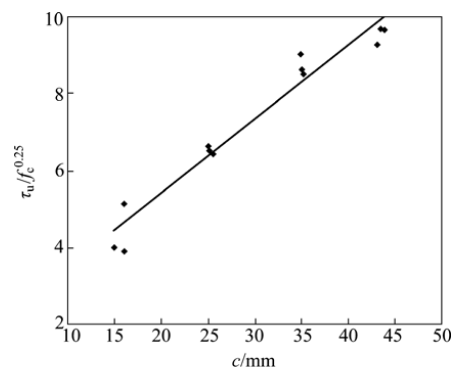
\includegraphics[width=0.6\textwidth]{tensile vs c.png}
    \caption{Relationship between concrete tensile strength and concrete cover \parencite{liTensileBondAnchorage2012}.}
    \label{fig:tensile_cover}
\end{figure}

\subsubsection{Embedment Length}
Average bond stress decreases as embedment length increases, because bond stress is non-uniformly distributed and the more remote portions of the bar contribute less to resistance. \textcite{liTensileBondAnchorage2012} confirmed this inverse relationship through their Group EL tests, expressing it as:

\begin{equation}
\frac{\tau_u}{{f^{\prime}_{c}}^{0.25}} = \frac{16.908d}{l_a}+4.8974
\end{equation}

They also noted the important practical upper limit: if embedment is too long, the bar yields or fractures before bond failure, the fully developed condition that represents the design objective of development length provisions.

\begin{figure}[H]
    \centering
    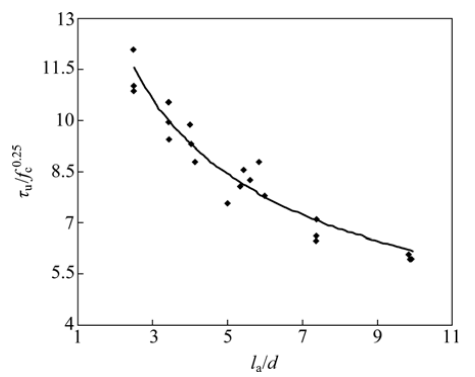
\includegraphics[width=0.6\textwidth]{tensile vs Lemb.png}
    \caption{Relationship between concrete tensile strength and embedment length \parencite{liTensileBondAnchorage2012}.}
    \label{fig:tensile_lemb}
\end{figure}

\subsubsection{Transverse Confinement}
Transverse reinforcement (stirrups or helices) confines the propagation of longitudinal splitting cracks, resisting both vertical and horizontal splitting and allowing higher rib bearing forces to develop before failure. \textcite{liTensileBondAnchorage2012} demonstrated that stirrups can significantly enhance bond strength, expressing the relationship as:

\begin{equation}
\frac{\tau_u}{{f^{\prime}_{c}}^{0.75}} = 33.057\frac{A_{sv1}}{cs_{sv}}+0.8852
\end{equation}

where $A_{sv1}$ is the stirrup bar area, $c$ is cover, and $s_{sv}$ is stirrup spacing. The use of ${f_{c}^{\prime }}^{0.75}$ rather than ${f_{c}^{\prime }}^{0.25}$ for unconfined bars, reflects the ACI 408R-03 finding that transverse reinforcement engages the concrete in a stress state where strength scales with a higher power of compressive strength. An upper limit exists beyond which additional confinement produces no further bond strength increase, and bar pull-out or fracture governs instead. 

\begin{figure}[H]
    \centering
    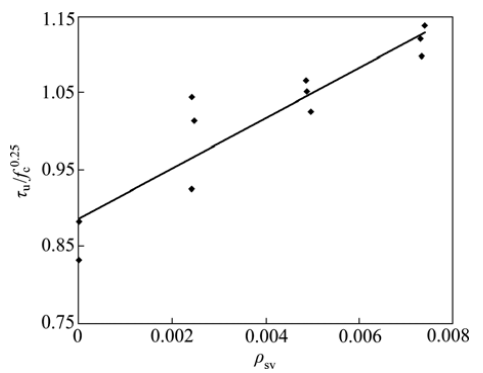
\includegraphics[width=0.6\textwidth]{tensile vs conf.png}
    \caption{Relationship between concrete tensile strength and transverse confinement \parencite{liTensileBondAnchorage2012}.}
    \label{fig:tensile_conf}
\end{figure}

\subsubsection{Bar Surface Geometry and Relative Rib Area}
The relative rib area $f_{R}$, the ratio of projected rib area perpendicular to the bar axis to the nominal bar surface area, quantifies the mechanical interlock efficiency of a deformed bar. Higher $f_{R}$ produces greater mechanical interlock per unit slip, increasing peak bond stress and reducing required development lengths. AS/NZS 4671:2019 specifies minimum $f_{R}$ values for Class N bars as a function of diameter. The SENSE600 bar's rib pattern was designed to exceed this minimum, providing a positive bond performance margin. \textcite{paulettaBondSlipBehaviorStainless2020} demonstrated that bars with different rib profiles, even within the broad category of deformed steel, cannot be assumed to follow the same bond-slip parameters without experimental recalibration, reinforcing the need for SENSE600-specific characterisation.

\subsection{Prediction Models}
The following models are reviewed in chronological order. They are selected because they form a direct theoretical and methodological lineage: Orangun, Jirsa and Breen (1977) provide the empirical regression framework that underpins all code development length expressions; Darwin et al./ACI 408R-03 (2003) provide the reliability-calibrated database analysis that identifies the limitations of the Orangun model and motivates key refinements; fib Model Code 2010 (Cairns, 2015) provides the current international benchmark that unifies the preceding work into a comprehensive semi-mechanical model; and Andreasen and Nielsen (1989) provide the plasticity-based anchorage framework directly used by Foster et al. (2024) to derive the SENSE600 development length equation, and which will be extended in the present thesis. Together, these five models encompass the full progression from empirical observation to mechanistically grounded prediction, and each build on the limitations of its predecessor.

\subsubsection{Orangun, Jirsa and Breen (1977) - The Foundational Empirical Regression}
Orangun, Jirsa and Breen (1977) represented the pivotal transition from working-stress allowable bond values to strength-based development length design. Using a large database of beam splice and pull-out tests, they derived a multivariate regression expressing normalised bond strength as:

\begin{equation}
\frac{u}{\sqrt{f'_c}} = 0.1 + 0.25\frac{c}{d_b} + 4.15\frac{d_b}{l_d} + \frac{A_{tr}f_{tr}}{500 s d_b}
\end{equation}

where $u$ is average bond stress at failure (MPa), $c$ is the governing cover dimension (mm), $l_{d}$ is development or splice length (mm), $A_{tr}$ is the total area of transverse reinforcement within spacing $s$ (mm), and $f_{tr}$ is the transverse reinforcement yield strength (MPa). The four terms capture: a baseline bond capacity; the benefit of cover (consistent with Tepfers' prediction); the inverse relationship between embedment length and average bond stress; and the confinement benefit of transverse reinforcement. Rearranging to solve for $l_d$ directly yielded the structural template for ACI 318 and AS3600 development length provisions that remains in use today.

Orangun et al. also established that development length should be designed with a capacity-reduction philosophy, treated as a strength limit state analogous to flexure or shear, rather than simply by inflating bar stress. The key limitation is the use of $\sqrt{f_{c}^{\prime }}$ as the concrete term, which overestimates the concrete contribution to bond for $f_{c}^{\prime }$ above approximately 40 MPa. This is addressed by Darwin et al. in Section 1.4.2.

\subsubsection{Darwin et al. / ACI Committee 408 (2003) - Database Reliability }
The work of Darwin and colleagues, culminating in ACI 408R-03 (2003), represents the most thorough analytical audit of the empirical development length literature. Compiling over 1,000 beam splice and pull-out specimens, the Committee applied formal reliability analysis to the ACI 318 provisions and identified three important findings.

First, and most significant for the present thesis: the concrete contribution to bond is more accurately represented by ${f_{c}^{\prime }}^{0.25}$  than by $\sqrt{f_{c}^{\prime }}$. Darwin (2005) showed through regression analysis of the full dataset that ${f_{c}^{\prime }}^{0.25}$ produces a substantially tighter and less biased fit across the range of 17–110 MPa. The physical explanation is that at higher concrete grades, fracture transitions from aggregate debonding (where strength scales with $\sqrt{f_{c}^{\prime }}$.) toward aggregate splitting (where matrix toughness grows more slowly), saturating the bond benefit of higher-strength concrete. \textcite{liTensileBondAnchorage2012} adopted this recommendation directly, using ${f_{c}^{\prime }}^{0.25}$ throughout all their regression expressions for Australian 500N bars.

Second, for bars confined by transverse reinforcement, the concrete contribution scales with a higher power, between ${f_{c}^{\prime }}^{0.75}$ and ${f_{c}^{\prime }}^{1.0}$,  because confinement engages the matrix in a stress state where aggregate friction and compression are more intensively mobilised. \textcite{liTensileBondAnchorage2012} reflected this in their stirrup regression by using ${f_{c}^{\prime }}^{0.75}$ for confined specimens, consistent with the Committee's recommendation.

Third, the ACI 318 provisions were shown to provide inconsistent reliability across bar sizes and cover conditions, unconservative in some cases (e.g., the 0.8 bar size factor for smaller bars, which was subsequently removed) and excessively conservative in others. The report recommended introducing an explicit $\phi$-factor for bond, analogous to those used for flexure and shear. 

\subsubsection{fib Model Code 2010 (Cairns, 2015) — Current International Benchmark}
The fib Model Code 2010, reviewed by Cairns (2015), represents the most comprehensive bond model currently codified in an international standard. It synthesises the empirical foundations of Orangun et al., the analytical splitting framework of Tepfers, and the reliability insights of ACI 408R-03 into a unified model that explicitly accounts for concrete strength, bar surface geometry, cover, transverse reinforcement, steel grade, and transverse confining pressure.

The basic design bond strength $f_{bd,0}$ is defined for benchmark conditions and modified by factors $\eta_1-\eta_4$:

\begin{equation}
    f_{bd,0}\ =\ {\eta }_{1}{\eta }_{2}{\eta }_{3}{\eta }_{4}\ \times \ (1/{\gamma }_{c})\ \times \ \sqrt{f_{ck}}
\end{equation}

where ${\eta }_{1}$ accounts for bond quality and casting position, ${\eta }_{2}$ for concrete strength relative to benchmark, ${\eta }_{3}$ for bar diameter (size effect), and most importantly ${\eta }_{4}$ for steel grade, ranging from 1.2 for 400 MPa steel down to 0.68 for 800 MPa steel. This explicit ${\eta }_{4}$ factor is the most significant analytical innovation of fib MC2010 relative to Orangun et al. and ACI 408R-03: it recognises that higher-grade bars have lower bond efficiency because the average bond stress mobilised over the longer required development length is reduced. For the present thesis, ${\eta }_{4}$ provides analytical justification for why a purpose-built bond model is needed for SENSE600 bars, the bond efficiency of a 600 MPa bar cannot be inferred from 500 MPa data by simple yield stress scaling.

The above equation was then calibrated using the ACI408 bond test database and validated using additional data gathers from fib TG4.5 to get a mean strength expression:

\begin{align}
f_{\mathrm{stm}}
&= 54\left(\frac{f_{\mathrm{cm}}}{25}\right)^{0.25}
     \left(\frac{25}{\phi}\right)^{0.2}
     \left(\frac{l_b}{\phi}\right)^{0.55}
     \left[
       \left(\frac{c_{\mathrm{min}}}{\phi}\right)^{0.25}
       \left(\frac{c_{\mathrm{max}}}{c_{\mathrm{min}}}\right)^{0.1}
       + k_m K_{\mathrm{tr}}
     \right] \label{eq:fstm} \\[6pt]
&\leq f_y \notag \\[6pt]
&\leq 10\sqrt{f_{\mathrm{cm}}}\,\frac{l_b}{\phi} \notag
\end{align}

\begin{figure}[H]
    \centering
    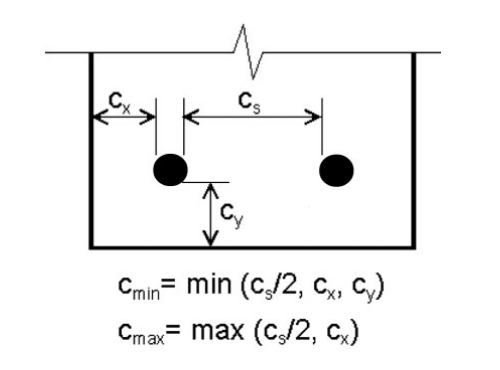
\includegraphics[width=0.6\textwidth]{conc cover.png}
    \caption{Definition of cover dimensions for fib MC2010 bond model \parencite{cairnsBondAnchorageEmbedded2015}.}
    \label{fig:conc_cover}
\end{figure}

\section{History of 500 MPa Reinforcement}

\subsection{Study on Australian 500N Bars}
\textcite{liTensileBondAnchorage2012} conducted a systematic experimental program characterising the tensile bond and anchorage properties of Australian-manufactured 500N Class reinforcing bars in concrete with compressive strengths from 25 to 65 MPa, using both pull-out specimens and beam anchorage tests. Their results demonstrated that AS 3600:2009 provisions were generally conservative for 500N bars across the tested range of concrete strengths and cover conditions, but that the degree of conservatism was variable, in some cases less than 10\%, which is insufficient for robust design given the inherent scatter in bond test data. The study also confirmed that the square root of compressive strength $\left(\sqrt{{f^{\prime }}_{c}}\right)$ adequately described the concrete contribution to bond for the 500N bars tested, though the authors noted that the fourth-root representation might be more accurate for higher concrete strengths.

\begin{figure}[H]
    \centering
    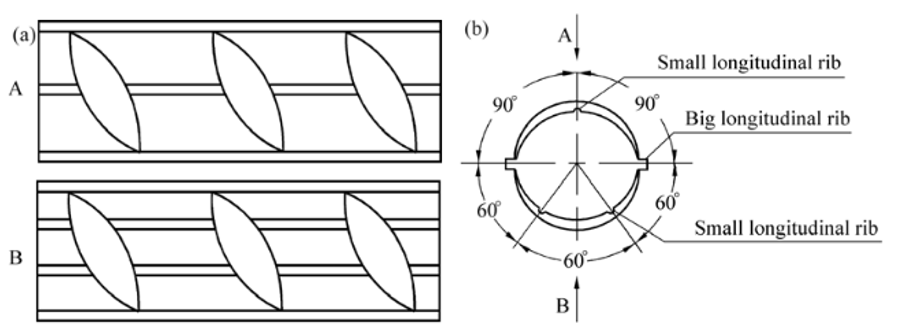
\includegraphics[width=0.8\textwidth]{500N rib pattern.png}
    \caption{Rib pattern of 500N Class reinforcing bars \parencite{liTensileBondAnchorage2012}.}
    \label{fig:500N_rib_pattern}
\end{figure}

This work remains the primary Australian experimental reference for 500 MPa bar bond behaviour and establishes the direct benchmark against which SENSE600 bond performance should be compared. The experimental methodology employed by Li et al., pull-out cylinders with helical confinement at multiple embedment lengths, across a range of concrete strengths, closely resembles the approach adopted by Foster et al. (2024) for SENSE600, enabling a direct comparison of bond performance between the two grades.

\subsection{Splice Strength and Lap Length for 500 MPa Bars}

Canbay and Frosch investigated the bond strength of lap-spliced bars, analysing existing test data to assess the reliability of ACI 318 lap splice provisions. They concluded that the modification factors used in ACI 318 for lap splices were based on limited and heterogeneous data and recommended a more unified approach in which splice strength is expressed directly as a function of development length without separate empirical multipliers. While their work was focused on 500 MPa class steel, the methodological framework is directly applicable to the derivation of lap splice provisions for SENSE600 bars. Similarly, Cairns (2015) reviewed the lap splice provisions in fib MC2010, noting that the model provides a more mechanistically transparent framework for splice design than empirical code multipliers, and that its calibration for higher steel grades required further experimental data.

Ahlborn, French and Shield (2000) demonstrated that bars with high relative rib area consistently achieved higher splice strengths than conventional bars of the same diameter, and that the advantage was most pronounced at shorter splice lengths — a finding with practical significance for the design of heavily congested connection zones where the shorter absolute lengths achievable with SENSE600 bars would be most beneficial.

\subsection{International Standards for 500 MPa and Beyond}
Internationally, the treatment of 500 MPa reinforcement in design codes has followed a consistent pattern: development length expressions from lower-grade calibration databases are scaled to 500 MPa using yield stress ratios, with the scaling validated through targeted experimental programs. Eurocode 2 (EN 1992-1-1:2004) accomodates yield strengths up to 600 MPa within its general development length framework, using the design bond stress $f_{bd}$ as the concrete capacity term and applying modification factors for cover and confinement. The fib Model Code 2010 similarly provides a general framework applicable to a range of yield strengths, though its bond-slip model parameters were primarily calibrated for 500 MPa class steel. ACI 318-19 provides development length expressions up to 550 MPa, beyond which code provisions are not directly applicable and independent experimental validation is required.

\section{Empirical Work on Development Lengths}
Empirical work on development length has progressed from simple average bond-stress concepts to more refined code-based formulations that attempt to represent confinement, bar geometry, steel grade, and stress state. Across the literature, the common mechanical basis is that development length is the embedment required to transfer steel force into the surrounding concrete without bond failure. Cairns (2015) notes that this can be expressed through the average bond relation:

\begin{equation}
    f_{b}\ =\ \frac{\Delta f_{s}A_{s}}{\pi \phi l_{b}}
\end{equation}

but stresses that this is only a convenient simplification because actual bond transfer is governed by rib bearing, splitting resistance, cover, spacing, and confinement rather than by a uniform interface shear stress alone. This chapter reviews what development length is, traces the progression of empirical and analytical models from the classic Orangun et al. regression to the current major code provisions, and concludes with the most recent Australian contribution, the Foster et al. (2024) development length equation for SENSE600 bars.

\subsection{What is development length?}

Development length is the minimum embedment length required for a reinforcing bar to develop its design yield strength at a critical section without bond failure occurring between the bar and the surrounding concrete. It is the macroscopic expression of the bond-slip constitutive relationship, translated into a single design length through integration of the local bond resistance over the bar's perimeter and embedment length.
The conceptual basis is straightforward: at a critical section, the reinforcing bar must carry its full design stress $\left(f_{sy}\right)$. For this stress to be developed, the force in the bar ($A_{s}\ \times \ f_{sy}$) must be transferred into the concrete through bond over the available embedment length. If the embedment is shorter than the development length, bond failure will occur before yield is reached, and the bar is unable to fulfil its structural role. Mathematically, the development length is derived from the equilibrium of the bar force and the total bond resistance:

\begin{equation}
    A_{s}\ \times \ f_{sy}\ =\ {\tau }_{avg}\ \times \pi \ \times \ d_{b}\ \times \ L_{sy.t}
\end{equation}

Rearranging, the development length is:

\begin{equation}
    L_{sy.t}\ =\frac{A_{s}\times \ f_{sy}}{{\tau }_{avg}\times \ \pi \ \times \ d_{b}}=\frac{d_{b}\times \ f_{sy}}{4{\tau }_{avg}}\ 
\end{equation}

The challenge in code development has always been the accurate determination of ${\tau }_{avg}$ the average bond stress mobilised over the development length at the point of bar yielding, which depends on concrete strength, cover, bar geometry, and confinement in ways that are not captured by a single constant. The entire history of development length research can be read as successive attempts to improve the prediction of ${\tau }_{avg}$ across the full range of design conditions.

A useful way to frame the analytical literature is to distinguish between older empirical development-length expressions and newer code formats derived from semi-mechanical bond models. The classic Orangun, Jirsa and Breen (1977) work remains important because it explicitly linked development length to bar stress, concrete strength, bar diameter, cover, and transverse reinforcement. They argued that development length should be treated with a capacity-reduction philosophy — not simply by inflating bar stress — because bond is a strength problem like flexure or shear. Their proposed regression directly informed ACI 318 and remains the methodological ancestor of all current code provisions.

\subsection{fib Model Code 2010}
Within the fib framework, the 2010 Model Code represents a significant analytical shift toward a mechanistically grounded bond model. Cairns (2015) explains that fib MC2010 first defines a basic design bond strength $f_{bd,0}$ for benchmark conditions and then modifies it for cover, transverse reinforcement, and transverse pressure. One of the most important changes relative to earlier codes is the explicit inclusion of steel grade through factor ${\eta }_{4}$, with values reducing from 1.2 for 400 MPa steel to 0.68 for 800 MPa steel. This reflects the physical reality that as yield strength increases, the development length required to reach bar yield also increases, so the average bond stress mobilised over that longer length is lower. In other words, fib MC2010 recognises analytically that higher steel grades cannot be treated using the same bond benchmark as lower-grade bars, a principle directly relevant to the SENSE600 context.

For straight bars in tension, Cairns (2015) reproduces the fib Model Code 2010 design bond strength as Equation 9:

\begin{equation}
    f_{bd}\ =\ \left({\alpha }_{2}\ +\ {\alpha }_{3}\right)f_{bd,0}\ -\ 2p_{tr} <  \ 2.0f_{bd,0}\ -\ 0.4p_{tr}\ \leq \ 1.5/{\gamma }_{c} \sqrt{f_{ck}}
\end{equation}

where ${\alpha }_{2}$ accounts for the effect of concrete cover and bar spacing on the splitting resistance, ${\alpha }_{3}$ accounts for the contribution of transverse reinforcement, $f_{bd,0}$ is the basic design bond strength for benchmark conditions (proportional to $\sqrt{f_{ck}}/{\gamma }_{c}$, with the steel grade factor ${\eta }_{4}$ incorporated), and $p_{tr}$ is the average compressive stress perpendicular to the bar axis (taken as positive in compression). Because transverse compression increases confining pressure and thereby enhances bond strength, a compressive $p_{tr}$ reduces the required anchorage length, one of the key conceptual advances in fib MC2010 relative to its predecessors.

Cairns (2015) argues that this is one of the most important conceptual changes in fib MC2010: shorter anchorages are no longer justified by a blanket distinction between anchorage and lap splice conditions, but by whether a beneficial transverse compression field is present. This distinction has direct practical relevance for the design of SENSE600 bar anchorages in regions of transverse compression (e.g., within beam-column joints or at well-confined supports) versus regions without beneficial compression (e.g., simply supported beam ends with minimum cover).
The basic design anchorage length in fib MC2010 is then derived from the equilibrium condition: 

\begin{equation}
    l_{bd}=\frac{A_{s}\ f_{sd}}{\pi \ d_{b}\ f_{bd}}
\end{equation}

where $f_{sd}$ is the design bar stress. For bars stressed to their design yield strength, this gives 

\begin{equation}
    l_{bd}=\frac{d_{b}f_{yd}}{4f_{bd}}
\end{equation}

which is the direct application of the average bond stress concept introduced in Section 3.1, but with $f_{bd}$ now rigorously derived from the bond-slip model and the confinement conditions of the specific design situation.

\subsection{Eurocode 2 (EN 1992-1-1:2004, Clause 8.4.4)}

Eurocode 2 (EN 1992-1-1:2004) treats the design anchorage length for straight bars in tension through a clearly structured sequence in Clause 8.4, culminating in the design anchorage length expression in Clause 8.4.4. The approach retains the classical 'basic required length plus modification factors' framework but embeds the same underlying bond mechanics as fib MC2010.

The starting point is the ultimate design bond stress (Clause 8.4.2):

\begin{equation}
    f_{bd}=2.25\ {\eta }_{1}{\eta }_{2}f_{ctd}
\end{equation}

where ${\eta }_{1}$ accounts for bond conditions and casting position (1.0 for good bond; 0.7 for poor bond, including top-cast bars with more than 250 mm of concrete below), ${\eta }_{2}$ accounts for bar diameter (1.0 for $d_b$ $\leq$ 32 mm; (132 $-$ $d_b$)/100 for $d_b$ $>$ 32 mm), and $f_{ctd}$ is the design tensile strength of concrete. The use of concrete tensile strength, rather than compressive strength, reflects the mechanistic reality that splitting failure, which governs bond in most practical situations, is fundamentally a tensile fracture problem.

The basic required anchorage length (Clause 8.4.3) for a straight bar stressed to its design value ${\sigma }_{sd}$ is then:

\begin{equation}
    l_{b,rqd}=\frac{d_{b}}{4}\times \frac{{\sigma }_{sd}}{f_{bd}}
\end{equation}

The design anchorage length (Clause 8.4.4) applies a set of modification factors to $l_{b,rqd}$:

\begin{equation}
    l_{bd}=\ {\alpha }_{1}{\alpha }_{2}{\alpha }_{3}{\alpha }_{4}{\alpha }_{5}\times \ l_{b,rqd}\ \geq  l_{b,min}
\end{equation}

where: ${\alpha }_{1}$ accounts for bar shape (1.0 for straight bars); ${\alpha }_{2}$ accounts for the effect of minimum concrete cover ($c_{d}/d_{b}$, limited to a minimum product ${\alpha }_{2}{\alpha }_{3}{\alpha }_{5}$ $\geq$ 0.7); ${\alpha }_{3}$ accounts for confinement by transverse reinforcement not welded to the main bar; ${\alpha }_{4}$ accounts for welded transverse bars along the design anchorage length; and ${\alpha }_{5}$ accounts for the effect of transverse compressive pressure along the design anchorage length. The minimum anchorage length is:

\begin{equation}
    l_{b,min}=max \left\{\ 0.3\times l_{b,rqd}\ ; \ 10d_{b}\ ;100\ mm\right\}
\end{equation}

This minimum ensures a practical lower bound on anchorage length regardless of the degree of confinement. The Eurocode framework is applicable for yield strengths up to 600 MPa and is therefore directly relevant to SENSE600 bar design in Australian bridge projects governed by European-derived specifications. Its explicit use of concrete tensile strength in the bond stress expression aligns it more closely with the mechanics of splitting failure than the $\sqrt{{f_{c}}^{\prime }}$ formulations used in ACI 318 and AS 3600.

\subsection{AS3600:2018 - Anchorage Chapter}

AS 3600:2018 Clause 13.1 governs development length in Australian building practice. The tension development length is:

\begin{equation}
    L_{sy.tb}\ =\ \frac{0.5 k_{1} k_{3} f_{sy}\ d_{b}}{k_{2} \sqrt{f_{c}^{\prime }}}\ \geq \ 0.058 f_{sy}k_{1}d_{b}
\end{equation}

Where:

$k_{1}$ = 1.3 for top-cast bars ($>$ 300 mm of concrete below), 1.0 otherwise
$k_{2}$ = (132 - $d_{b}$)/100
$k_{3}$ = 1.0 - 0.15($c_{d}$ - $d_{b}$)/ $d_{b}$ (cover factor, $0.7 \leq k_{3} \leq 1.0$).

Compression development is shorter because end bearing contributes to force transfer; no bar position factor applies. Both expressions use $\sqrt{f_{c}^{\prime }}$  despite ACI 408R-03 and Li et al. (2012) showing ${f_{c}^{\prime }}^{0.25}$ is more accurate above 40 MPa. Ng et al. (2024) showed that substituting equivalent-capacity SENSE600 bars into the tension expression increases predicted development lengths by 2.5 – 9.5\%, because the higher yield strength (×1.2) outweighs the reduced diameter (×0.913), the analytical finding that motivated Foster et al. (2024) to develop an improved-rib bar and purpose-built equation.

\subsection{AS5100.5:2017 - Anchorage Chapter}

AS5100.5 governs concrete bridge design in Australia and adopts the same core tension development length expression as AS3600:

\begin{equation}
    L_{sy.tb}\ =\ \frac{0.5 k_{1} k_{3} f_{sy}\ d_{b}}{k_{2} \sqrt{f_{c}^{\prime }}}\ \geq \ 0.058 f_{sy}k_{1}d_{b}
\end{equation}

Section 13 was substantially revised in 2017 to treat development length as a discrete analytical design problem, with separate clauses for tension, compression, headed bars, mesh, bundled bars, and lap splices, mirroring the AS 3600 structure. The bridge code supplements these provisions with requirements for fatigue, durability, and stress-reversal detailing relevant to live load cycling. For SENSE600 applications, the same equivalent-capacity substitution approach permitted under the 2024 amendments to AS 3600 and AS/NZS 4671 would apply.

\subsection{ACI 318-19 — Chapter 25.4 and Table 25.4.2.3}

ACI 318-19 places development length provisions for deformed bars in tension in Chapter 25.4.2, with the detailed tabulated expressions in Table 25.4.2.3. The ACI approach uses a simplified two-formula format depending on bar size and confinement conditions, derived from the Orangun et al. (1977) regression database and refined through the ACI 408R-03 reliability analysis. The general expression for development length is:

\begin{equation}
    l_{d}=\frac{3f_{y}{\psi }_{t}{\psi }_{e}{\psi }_{s}}{40\lambda \ \sqrt{f_{c}^{\prime }}\times \frac{c_{b}+\ K_{tr}}{d_{b}}} \times d_{b}
\end{equation}

where ${\psi }_{t}$ is the reinforcement location factor (1.3 for top bars; 1.0 otherwise), ${\psi }_{e}$ is the epoxy coating factor (1.5 for coated bars with cover $<$ 3$d_{b}$ or clear spacing $<$ 6$d_{b}$; 1.2 for other coated bars; 1.0 for uncoated), ${\psi }_{s}$ is the bar size factor (0.8 for No. 6 (19 mm) and smaller; 1.0 for larger), $\lambda$ accounts for lightweight concrete (0.75 for all-lightweight; 0.85 for sand-lightweight; 1.0 for normalweight), and ($c_{b}\ +\ K_{tr})/d_{b}$ is the confinement term, limited to a maximum of 2.5, where $c_{b}$ is the smaller of the distance from bar centre to nearest concrete surface and half the centre-to-centre bar spacing, and $K_{tr}\ =\ 40A_{tr}/sn$ is the transverse reinforcement index.

Table 25.4.2.3 of ACI 318-19 simplifies this expression into a tabulated format for two common design cases (a) bars with sufficient cover and spacing (or with minimum stirrups) and (b) other cases as reproduced in Table 1.3.1 below:

% Table
\begin{table}[H]
  \centering
  \caption{Simplified development length for deformed bars in tension (adapted from ACI 318-19 Table 25.4.2.3)}
  \label{tab:aci_ld}
  \renewcommand{\arraystretch}{1.4}
  \begin{tabularx}{\textwidth}{|>{\centering\arraybackslash}m{3cm}|C|C|C|}
    \hline
    \textbf{Condition} &
    Clear spacing $\geq d_b$, cover $\geq d_b$, stirrups $\geq$ minimum &
    Clear spacing $\geq 2d_b$, cover $\geq d_b$ (no stirrups required) &
    \textbf{Other cases} \\
    \hline
    \fstrut $d_b \leq 19$~mm (No.~6 bar and smaller) &
    $l_d = \dfrac{f_y \psi_t \psi_e}{25\lambda\sqrt{f'_c}} \times d_b$ &
    $l_d = \dfrac{f_y \psi_t \psi_e}{25\lambda\sqrt{f'_c}} \times d_b$ &
    $l_d = \dfrac{3 f_y \psi_t \psi_e}{50\lambda\sqrt{f'_c}} \times d_b$ \\
    \hline
    \fstrut $d_b \geq 22$~mm (No.~7 bar and larger) &
    $l_d = \dfrac{3 f_y \psi_t \psi_e}{50\lambda\sqrt{f'_c}} \times d_b$ &
    $l_d = \dfrac{3 f_y \psi_t \psi_e}{50\lambda\sqrt{f'_c}} \times d_b$ &
    $l_d = \dfrac{9 f_y \psi_t \psi_e}{100\lambda\sqrt{f'_c}} \times d_b$ \\
    \hline
  \end{tabularx}

  \smallskip
  \begin{minipage}{\textwidth}
    \footnotesize\itshape
    Adapted from ACI 318-19 Table 25.4.2.3. All expressions produce $l_{d}$ in mm when $f_{y}$ and $f_{c}^{\prime }$ are in MPa and $d_{b}$ is in mm. Minimum $l_{d} = 300$ mm.
  \end{minipage}
\end{table}

The ACI 318-19 provisions apply to bars with yield strengths up to 550 MPa (80 ksi). For higher-grade bars, ACI 318 currently requires that development length be determined through alternative methods, such as the ACI 408R approach or testing, because the code provisions have not been validated beyond this range. This gap directly parallels the situation for SENSE600 bars in Australian practice prior to the Foster et al. (2024) experimental program.

The ACI Committee 408 report (ACI 408R-03) provides important analytical context for the ACI 318 provisions. The report argues that bond is a structural property, not a simple material property, and that empirical development length equations must reflect confinement, bar geometry, and realistic splice lengths. ACI 408R-03 concludes that the concrete contribution to bond is better represented by ${f_{c}^{\prime }}^{0.25}$ than by ${f_{c}^{\prime }}^{0.5}$, and it rejects the 0.8 bar-size factor for smaller bars as unjustified once realistic development lengths are considered. These recommendations have not yet been adopted in ACI 318-19, but they are reflected in the Li et al. (2012) composite bond strength formula (where ${f_{c}^{\prime }}^{0.25}$ is used) and are relevant to the calibration of the SENSE600 development length equation.

\subsection{Foster et al. (2024) - SENSE600 Development Length Equation}

Foster et al. (2024) represent the most recent and directly applicable contribution to the analytical development length literature for the Australian context. Building on the Andreasen and Nielsen (1989) plasticity-based anchorage model reviewed in Chapter 1, and validated against 54 pull-out tests on InfraBuild SENSE600 bars from 9.8 to 36.5 mm in diameter at a concrete strength of approximately 32.8 MPa, they proposed the following development length equation for Grade 600 SENSE600 bars:

\begin{equation}
L_{sy.tb}\ =\ \frac{270 k_{1} k_{3} d_{b}}{k_{2} \sqrt{f_{c}^{\prime }}}\ \geq \ 31.6 k_{1}d_{b}
\end{equation}

where $k_{1}$,$k_{2}$ and $k_{3}$ are as defined in AS 3600:2018. This equation adopts the existing AS 3600 modification factor framework to facilitate integration with Australian code practice, with the numerical coefficient 270 (compared to the AS 3600 coefficient of 0.5 × $f_{sy}$ = 0.5 × 500 = 250 for 500 MPa bars at benchmark conditions) reflecting the higher yield strength of the SENSE600 bar.

The analytical significance of the equation is considerable. Foster et al. demonstrated experimentally that an embedment of $16.2d_{b}$ is sufficient to develop the nominal yield strength of 600 MPa (with a factor of safety of 1.4 relative to the $\phi$-reduced stress), while $23d_{b}$ consistently causes bar fracture, confirming that the design equation provides an appropriate margin between yield development and bar fracture. Direct comparison with AS 3600:2018 requirements for equivalent-capacity Grade 500 bars showed that smaller-diameter Grade 600 SENSE600 bars can replace Grade 500 bars without requiring longer absolute development lengths, maintaining similar factors of safety against bond failure and bar splitting.

However, Foster et al. explicitly acknowledged that the equation was derived from tests at a single concrete strength ($f_{c}\prime  \approx 33 MPa$) and a single transverse reinforcement configuration and does not capture the variation in bond performance with concrete strength, cover geometry, and bar size that a complete bond model would provide. This limitation is the central analytical gap addressed by the present thesis.

\section{Analytical Work on Development Length}

The empirical and code-based development length expressions reviewed in the previous section are fundamentally regression models: they distil large experimental datasets into compact formulae calibrated to a specific range of material grades, bar geometries, and concrete strengths. While this approach is practically convenient and has served the industry reliably for 500 MPa class reinforcement, it carries an inherent limitation when bar grade, rib geometry, or concrete strength fall outside the calibration range, there is no mechanistic basis for extrapolation. The development of a bond model and development length equation for SENSE600 bars confronts precisely this limitation. Meeting it requires an analytical framework capable of predicting bond behaviour from first principles, representing the geometry of the bar-matrix interface, the stress state of the surrounding material, and the physical conditions under which failure initiates.

\subsection{The Volkersen Shear-Lag Model - Analytical Baseline}
The earliest and most enduring analytical approach to force transfer in adhesively bonded and embedded rod systems is the shear-lag model proposed by Volkersen (1938). The model treats the embedded rod and its surrounding matrix as two elastic adherends connected by a shear-only interface layer and derives the shear stress distribution along the bond length from a differential equilibrium argument. For a cylindrical bonded assembly, structurally analogous to a reinforcing bar embedded in concrete, Gustafsson and Serrano (2001) extended Volkersen's formulation to express the pull-out load capacity as:

\begin{equation}
    \frac{P_{f}}{2\pi rLf_{v}^{A}}=\frac{G_{f}\omega E_{s}A_{s}}{\pi rLf_{v}^{2A}}\left(\frac{\tanh{\left(\omega L\right)}}{1+E_{s}A_{s}/E_{t}A_{t}}\right)
\end{equation}

where $G_{f}$ is the fracture energy, ${f_{v}}^{A}$ is the bond interface shear strength, $G_{A}$ the shear modulus of the interface layer, $r_{s}$ and $r_{A}$ the rod and interface radii, $E_{s}$ and $E_{t}$ the rod and matrix elastic moduli, and $A_{s}$ and $A_{t}$ the respective cross-sectional areas (Gustafsson and Serrano, 2001). 

The shear stress concentration is highest at the loaded end and diminishes exponentially toward the free end, consistent with the experimental observation that bond failure initiates at the loaded end and propagates along the embedment (Alavi et al., 2025).

Despite its widespread adoption, the Volkersen model has well-documented limitations. Alavi et al. (2025) validated the model against pull-out tests on glued-in rod (GiR) timber joints across embedment lengths of 80–360 mm and found that the Volkersen model consistently overestimated pull-out capacity by margins of 35–122\% relative to experimental failure loads. Three physical deficiencies account for this overestimation. First, the model ignores all deformation of the adherends in the radial direction, meaning the radial (splitting) component of the interface stress, responsible for splitting failure in both GiR joints and reinforced concrete, is entirely absent from the formulation (Nemes and Lachaud, 2009; Alavi et al., 2025). Second, the influence of adherend deformation and the non-linearity of the adhesive are ignored, making the model applicable only to joints with a uniform overlap length and relatively thin adherends or adhesives (Alavi et al., 2025). Third, the model does not consistently yield accurate results when the load levels associated with different failure modes are not well separated; that is, when pull-out and splitting failure occur at similar load levels, because a single shear-only interface representation cannot capture the mode interaction (Alavi et al., 2025). The Volkersen model therefore provides a useful analytical baseline and comparative benchmark but cannot serve as the foundation for a rigorous development length model that must capture the pull-out/splitting mode transition.

\subsection{Elasticity-Based Cylindrical Stress Models}
\subsubsection{Nemes and Lachaud (2009) - Refined Cylindrical Assembly Model}

A significant advance over the Volkersen shear-lag approach was made by Nemes and Lachaud (2009), who developed a refined analytical model for the stress distribution in cylindrical adhesively bonded assemblies based on the variational principle of minimum complementary energy. Their model formulates all stress components, axial ($\sigma_{zz}$), circumferential ($\sigma_{\theta\theta}$), radial ($\sigma_{rr}$), and shear ($\tau_{rz}$), within the inner rod, adhesive layer, and outer matrix as functions of the axial stress $\sigma_{zz}^{(1)}(z)$ in the inner tube, using equilibrium equations in a cylindrical coordinate system $(z, r, \theta)$ and boundary conditions at each material interface (Nemes and Lachaud, 2009). Table 1 of Nemes and Lachaud (2009) shows that prior models — including their own earlier formulation, had assumed the radial stress to be zero; their refined model was the first in the cylindrical assembly literature to explicitly include $\sigma_{rr}$ as a non-trivial stress component.

Nemes and Lachaud (2009) assumed a linear variation of radial stress in each material:
\begin{align}
  \sigma_{rr}^{(1)} &= \alpha_1 \left[ r - r_i \right] \\
  \sigma_{rr}^{(c)} &= \beta = \text{constant} \\
  \sigma_{rr}^{(2)} &= \alpha_2 \left[ r - r_e \right]
\end{align}

where $r_i$ and $r_e$ are the inner and outer radii of the adhesive layer, and $\alpha_1$, $\alpha_2$, and $\beta$ are constants determined from boundary conditions. The axial stress in the inner rod is then related to the radial stress through the equilibrium equations, allowing for a complete resolution of the stress field in all three materials.

Substituting these radial stress expressions into the equilibrium equations and the potential energy integral, and applying variational calculus, yields a fourth order governing ordinary differential equation for $\sigma_{zz}^{(1)}(z)$ (Nemes and Lachaud, 2009):

\begin{equation}
    E\ \frac{d^{4}{\sigma }_{zz}}{dz^{4}}\ +\ \left(B - C\right)\frac{d^{2}{\sigma }_{zz}}{dz^{2}}\ +\ A\ {\sigma }_{zz}\ +\frac{D}{2}\ +\frac{{\alpha }_{1}k}{2}\ =\ 0\ 
\end{equation}

where $A$, $B$, $C$, $D$ and $E$ are integration constants depending on the elastic moduli, Poisson's ratios and radii of all three materials, and $k$, $h$ and $m$ depend on the load and dimensional specifications of the assembly \textcite{nemesModelingCylindricalAdhesively2009}. The general solution takes the form $\sigma_{zz}(z) = \sum_i B_i \exp(\omega_i z) + \text{constant}$, with integration constants determined from the loading boundary conditions at $z = 0$ and $z = L$.

The key result from the comparative study of Nemes and Lachaud (2009) was that incorporating radial stress has an important influence particularly on the distribution of the circumferential (hoop) stress ${\sigma }_{\theta \theta}$ in both the inner tube and the adhesive layer while having a more modest effect on the shear stress ${\tau }_{rz}$ distribution. Since hoop stress is the stress component directly responsible for splitting failure in both bonded rod systems and reinforced concrete, it is the hoop stress that drives longitudinal cracking through the cover in Tepfers' (1973) thick-walled cylinder model. This finding has a direct and important implication: any analytical bond model that ignores radial stress will misrepresent the component of the stress field most critical to the pull-out/splitting mode transition. The Nemes and Lachaud (2009) framework therefore provide the first analytical model suitable as a basis for predicting whether splitting or pull-out governs in a bonded cylindrical assembly.

\subsubsection{Alavi, Valipour and Bradford (2025) — Extended Model for GiR Timber Joints}

\textcite{alaviAnalyticalProcedureFailure2025} built directly on the \parencite{nemesModelingCylindricalAdhesively2009} framework to develop a comprehensive elasticity-based analytical model for single glued-in rod (GiR) timber joints subjected to pull-pull, pull-push, rod-pull, and wood-pull loading configurations. GiR joints, comprising a steel rod bonded into a timber element by adhesive, are structurally analogous to deformed reinforcing bars in concrete: in both systems a cylindrical rod embedded in a matrix material transfers axial force through interfacial shear and rib bearing. The analytical insights and solution methodology developed for GiR joints are therefore directly transferable to the reinforcing bar bond problem \parencite{alaviAnalyticalProcedureFailure2025}.

The model formulated the governing equations in a cylindrical coordinate system, treating the steel bar as isotropic and the timber as transversely isotropic (with distinct longitudinal $E_{l}$ and transverse $E_{t}$ elastic moduli, shear modulus $G_{12}$, and Poisson's ratio ${\nu }_{12}$). A key improvement over Nemes and Lachaud (2009) was the adoption of a non-linear radial stress distribution \parencite{alaviAnalyticalProcedureFailure2025}:
\begin{gather}
  \sigma_r^{s}(r) = \Lambda_1 r^2 \\
  \sigma_r^{A} = \Lambda_2 \\
  \sigma_r^{t}(r) = \Lambda_3 \left( r^2 - r_t^2 \right)
\end{gather}
where $\Lambda_i$ are constants determined from radial stress continuity at the rod--adhesive and adhesive--timber interfaces \parencite{alaviAnalyticalProcedureFailure2025}. Substituting these into the equilibrium equations yields the shear and hoop stress components in each material analytically as functions of the first and second derivatives of $\sigma_z^{s}(z)$. Introducing all stress components into the strain energy expression and applying the variational principle $\delta U = 0$ produces a fourth-order governing ODE for $\sigma_z^{s}(z)$ with coefficients $\Xi_1$ through $\Xi_7$ that incorporate the transversely isotropic timber properties \parencite{alaviAnalyticalProcedureFailure2025}. The general solution is:
\begin{equation}
  \sigma_z^{s}(z) = B_1 e^{\omega_1 z} + B_2 e^{-\omega_1 z} + B_3 e^{\omega_2 z} + B_4 e^{-\omega_2 z} + \wp
\end{equation}
where $\omega_1$ and $\omega_2$ are the characteristic roots of the ODE and $\wp$ is a particular solution depending on material properties, geometry and loading conditions. The four integration constants $B_1$--$B_4$ are determined by applying boundary conditions corresponding to each of the four loading configurations \parencite{alaviAnalyticalProcedureFailure2025}. Extending the analytical solution to all four loading configurations simultaneously was a key contribution, as prior analytical models had only addressed pull--pull and pull--push conditions.

The GiR joint stiffness is derived directly from the analytical solution via conservation of energy: setting external work equal to internal strain energy, 

\begin{equation}
k_{s}\ =\ \frac{f}{{\delta }_{z}^{s}}\ =\frac{f^{2}}{2U}
\end{equation}

yielding a closed-form expression for joint stiffness without the need for finite element analysis. Validation against detailed FE simulations showed that the non-linear radial stress formulation significantly improved accuracy relative to models assuming zero or linear radial stress. The proposed model achieved a stiffness prediction within 14\% of experimental values across rod radii of 4–6 mm and embedment lengths of 80–360 mm, whereas the Volkersen model overestimated failure loads by 35–122\% and the EN1995-1-1 code provisions grossly underestimated both failure load and stiffness \parencite{alaviAnalyticalProcedureFailure2025}.

The analytical framework of \textcite{alaviAnalyticalProcedureFailure2025}) is directly relevant to SENSE600 bond modelling for three reasons. First, the cylindrical geometry, isotropic steel rod, and force-transfer mechanism are structurally identical to those of a deformed reinforcing bar in concrete. Second, the non-linear radial stress formulation correctly captures the hoop stress that governs splitting failure — the dominant design concern for SENSE600 bars in slabs without transverse reinforcement. Third, the closed-form solution provides a basis for analytically deriving development length as a function of material properties and geometry, rather than empirical regression.

\subsection{Fracture Mechanics Failure Criteria}

\section{Background on SENSE600 Bars and the Australian Context}
\subsection{Introduction of 600 MPa Reinforcement in Australia}
The introduction of 600 MPa Class N reinforcing steel into Australian construction practice represents the latest step in the progressive evolution of reinforcement grade, following the transition from 400 to 500 MPa in the 1990s. In early 2024, following amendments to AS 3600:2018 and AS/NZS 4671:2019, 600 MPa Class N bars became available for structural use in Australia. The impetus for this development was primarily sustainability: by reducing bar cross-sectional area for the same tensile capacity, 600 MPa bars enable material savings of up to 17\% and embodied carbon reductions of approximately 39\% per tonne of steel placed, attributed to both lower mass and the use of recycled steel in electric arc furnace production (Foster et al., 2024).

The commercial product that has driven this development in Australia is the SENSE600 bar, manufactured by InfraBuild Australia. SENSE600 bars are produced in a range of diameters scaled to deliver equivalent force capacity ($A_s f_{sy}$) to standard 500 MPa bars of the next larger nominal size. The bars feature a proprietary optimised rib pattern, with increased relative rib area relative to standard 500 MPa Class N bars, designed to ensure that the smaller diameter SENSE600 bar achieves bond and development length performance equivalent to, or better than, the larger 500 MPa bar it replaces.

\subsection{AS/NZS 4671:2019 and Bar Geometry Requirements}
AS/NZS 4671:2019 specifies the mechanical and geometric requirements for reinforcing steel bars for structural use in Australia and New Zealand, including minimum yield strength, tensile strength, elongation at fracture, and relative rib area. For Class N bars, the minimum relative rib area $f_{R,min}$ increases with bar diameter, reflecting the greater embedment depth required for larger bars and the importance of maintaining adequate mechanical interlock. The SENSE600 bar's rib pattern was designed to exceed the minimum $f_{R}$ requirement, providing a positive bond performance margin over the code minimum. Ng and McGregor (2024) confirmed through measurement that the SENSE600 bar meets and exceeds the AS/NZS 4671:2019 relative rib area requirements across all tested diameters.

\subsection{Ng and McGregor (2024) - Stage I Experimental Program}
Ng and McGregor (2024) reported the Stage I experimental investigation of bond performance for InfraBuild SENSE600 bars, comprising 18 pull-out tests on bars with nominal equivalent diameters of 14.6, 21.9, and 29.2 mm (corresponding to 500 MPa equivalent sizes of 16, 24, and 32 mm). Tests were conducted at embedment lengths ranging from 13$d_b$ to 32$d_b$ in 25 MPa concrete confined by 5.4 mm diameter helical reinforcement. The key outcome was that an embedment length of approximately $22d_b$ was required to achieve the code criterion of 0.2 mm free-end slip at the nominal yield stress of 600 MPa, while 32$d_b$ consistently produced bar fracture, confirming full anchorage. The improved rib pattern was shown to deliver bond performance equivalent to standard 500 MPa bars of the equivalent force capacity, validating the design concept.

The Stage I program, while important as proof-of-concept, was limited by its use of a single concrete strength (nominally 25 MPa), a single transverse reinforcement configuration, and only three bar diameters. These limitations motivated the more comprehensive Stage II program reported by Foster et al. (2024) and underscore the need for a broader experimental database from which a generalised bond model can be derived.

\subsection{Foster et al. (2024) - Stage II Experimental Program and Development Length Equation}

Foster, Ng, McGregor, and Valipour Goudarzi (2024) presented the Stage II experimental program, extending the dataset to 54 pull-out specimens across six bar sizes (nominal diameters 9.8 to 36.5 mm), all tested at an embedment length of 20db in concrete with a mean compressive strength of 32.8 MPa, confined by 5.4 mm helical reinforcement. All specimens achieved or exceeded the nominal yield strength of 600 MPa at 20db, with stresses at 0.2 mm free-end slip ranging from 671 to 784 MPa — all above the mean 600 MPa yield threshold. At failure, bar stresses were at or near the ultimate tensile strength, confirming that 20db represents the transition point between bond failure and bar fracture for this configuration.

A plasticity-based analytical model, adapted from the Andreasen and Nielsen (1989) upper- and lower-bound plasticity framework, was calibrated against the combined Stage I and II dataset and showed good agreement with the experimental results. The model characterises anchorage strength as:

\begin{equation}
{\sigma }_{b}=\eta \ f_{c}\left(\frac{l_{b}}{d_{b}}\right)
\end{equation}

where $\eta$ is a non-dimensional parameter dependent on bar rib geometry, concrete efficiency, and confinement level. Based on the experimental program and analytical model, Foster et al. (2024) proposed the development length equation seen above. The equation adopts the existing AS 3600 framework to facilitate code integration and was validated at $f_{c} \approx 33 MPa$.

The authors explicitly acknowledged the key limitation of the proposed equation: it is based on a single concrete strength and a single confinement configuration. A validated bond model capable of predicting development length across the full range of concrete strengths (25–65 MPa) and cover conditions encountered in Australian practice, and from which the development length equation can be derived analytically, remains an outstanding research need. This is the central gap that the present thesis aims to close.

\subsection{Ng and McGregor (2024) - Changes to Australian Standards}
In a complementary paper, Ng and McGregor (2024) reviewed the changes to AS 3600:2018 and AS/NZS 4671:2019 required to accommodate higher-strength reinforcing steels, situating the SENSE600 development within the broader context of international trends toward 600 MPa and higher-grade reinforcement. They documented the technical rationale for the equivalent force capacity substitution approach in which a 600 MPa bar of diameter $d_{b}$ replaces a 500 MPa bar of diameter $d_{b}$ and discussed its implications for development length, lap splice design, and structural detailing. The paper reinforced the conclusion that while the substitution approach is technically sound as a first approximation, purpose-built bond model and development length provisions for SENSE600 bars would provide a more rigorous and flexible design basis.

\section{Summary and Research Gap}
\subsection{Summary}

\subsection{Research Gap}